\subsection{Will I get the dukedom promised by the King?}
\begin{frame}[t]{Will I get the dukedom promised by the King? [JH p57] [RH p59,80-82]}
\begin{columns}[T, onlytextwidth]
\column{0.5\textwidth}
\footnotesize
\Jupiter\ is L1, in the 10th (house of rulers)\\
\hspace{1em}he aspects his domicile  (\Sagittarius) on the 1st; \\
\hspace{1em}he will get his dukedom \\
\Jupiter\ in detriment in \Virgo\\ 
\hspace{1em}detriment indicates a "flawed" dukedom, \\
\hspace{1em}not "no" dukedom \\
\Sun\ \& \Venus\ (connected to 1st) $\Rightarrow$ to \Square\ of \Sagittarius\ in 1st (received) \\
\hspace{1em}supports a "yes", he will get his dukedom\\
\vspace{0.5em}
\Mercury\ is L7, retro, a rebel opponent in the matter \\
\hspace{1em}cadent in the 12th \\
\hspace{1em}$\Rightarrow$ \Opposition\ \Saturn\ retro, cadent and without reception \\
\hspace{1em}disposited by \Venus, combust, which worsens matters \\
\hspace{1em}indicating destruction for the opponent \\
\vspace{0.5em}
\Mercury\ retro, by transit, $\Rightarrow$ \Sextile\ \Jupiter\ with reception indicates the rebel opponent will end by seeking "peace and accommodation" from the querent

\column{0.5\textwidth}
\begin{center}
{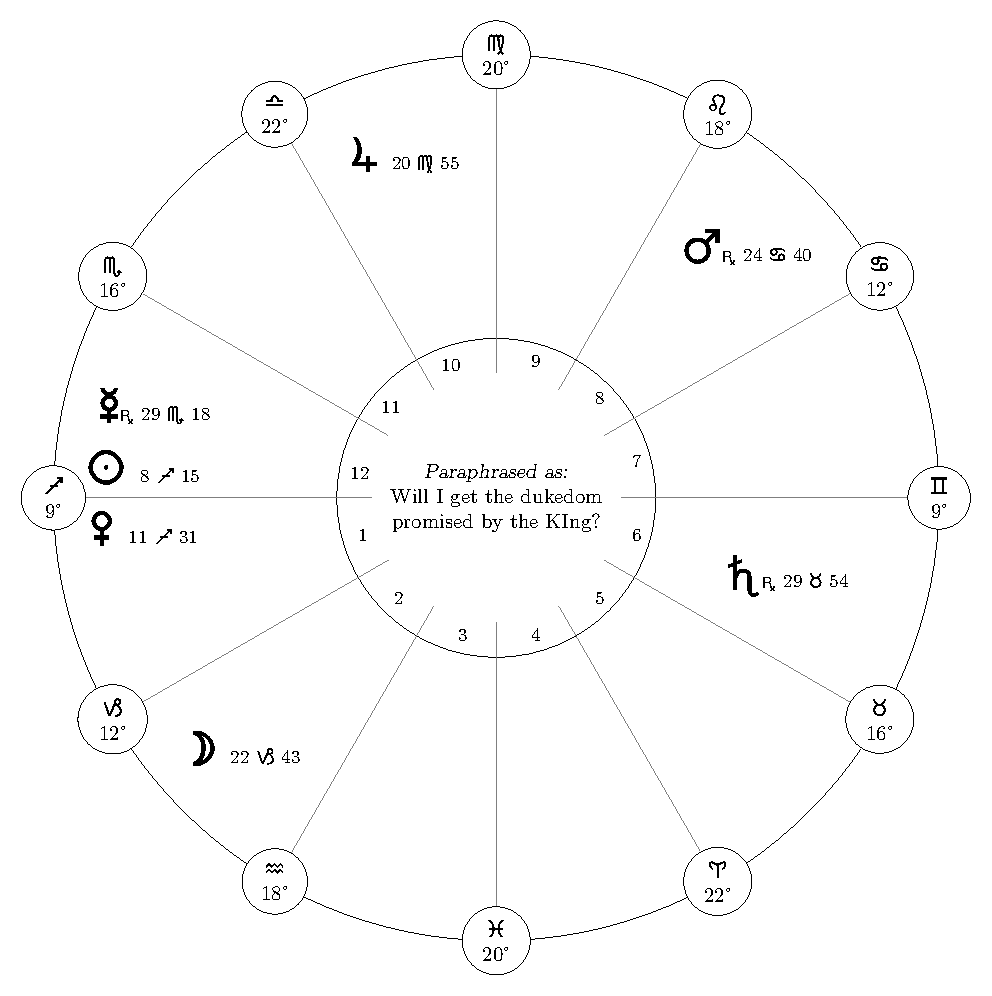
\includegraphics[width=0.9\textwidth]{charts/52-chart-dukedom}} \\
\scriptsize
The MC was not given, only the Asc degree. The other cusps are in the text Holden used but are not original to Masha'Allah.
\end{center}
\end{columns}

\end{frame}
% --------------------------------------------------------------
\begin{frame}[t]{Dukedom Chart as Battle Chart}
\footnotesize
\begin{columns}[T, onlytextwidth]
\column{0.5\textwidth}
Masha'allah goes further into the chart, reading it as a 'battle' or 'war' chart; he begins with the \Moon, using its separating to identify the querent and its application to identify the rebel lord. \\
\vspace{0.25cm}
\Moon\ separating \Trine\ \Jupiter\ (reinforces \Jupiter\ as main significator) \\
\Moon\ applying \Opposition\ \Mars\ in \Cancer\ (mixed reception) \\
\vspace{0.2cm}
\Mars\Retrograde, in 8th, in his Fall (\Cancer); indicates the opponents penury (8th is 2nd from 7th) \\
\vspace{0.2cm}
\Moon\ dispositing \Mars\ is in 2nd, querent's resources \\
The rebel lord could not pay his army so the querent bought them off; ending the battle \\
\vspace{0.25cm}
But, as \Mars\ is the dispositor of \Mercury\ (L7), and it is in a strong reception with the \Moon, the rebel lord will not lose everything and, as already noted, \Mercury\ to the \Sextile\ to \Jupiter\ indicates a peaceful conclusion for all involved.\\
\vspace{0.2cm}
This is the last of Masha'allah's examples.
\column{0.5\textwidth}
\begin{center}
{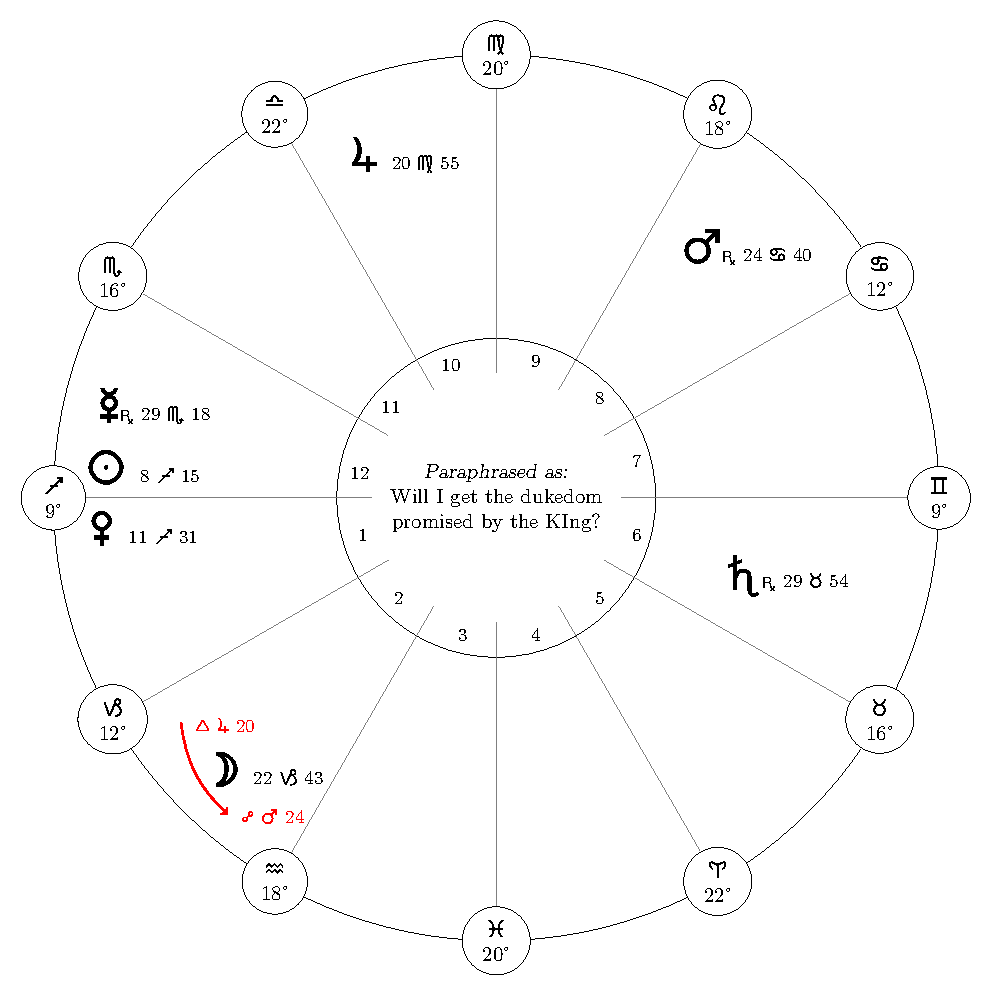
\includegraphics[width=0.9\textwidth]{charts/52a-chart-dukedom}} \\
\end{center}
\end{columns}
\end{frame}